% 結果の章（数値は 図/values.tex と 図/tab_*.tex から。手で書かない）

% ============================================================
\chapter{主な検定}\label{ch:primary}

\begin{table}[H]
\centering\small
\caption{主な検定 P：2020 年以降・範囲の中の発表で、2〜60 取引日の変動率（対数）を \code{chrono\_risk} と統制・固定効果で回帰した結果}
\label{tab:primary}
\begin{tabular}{@{}lr@{}}
\toprule
点数が 1 標準偏差高いときの変動率の差 & \V{Pcoef}\V{Punit} \\
95\% 信頼区間 & [\V{Plo}, \V{Phi}]\V{Punit} \\
$t$（反応日ごとにまとめた標準誤差） & \V{Pt} \\
片側 $p$ & \V{Pp} \\
置換（同じ反応日の中で 1,000 回）の片側 $p$ & \V{Pperm} \\
発表の数（反応日の数） & \V{Pn}（\V{Pdates}） \\
決定係数の増分 & \V{Prtwo} ポイント \\
\midrule
判定 & \textbf{\V{Pverdict}} \\
\bottomrule
\end{tabular}
\end{table}

\begin{keybox}[結果]
事前登録の判定の基準を両方とも満たし、仮説は\textbf{支持}された。ChronoGPT＋リッジの点数が 1 標準偏差高い発表は、発表の前の変動率（2 つの期間）・2 日の反応の大きさ・規模・驚きの大きさ・業種と時期の固定効果を統制したうえで、その後 2〜60 取引日の変動率が \V{Pcoef}\V{Punit} 高かった。1,000 回の置換のどれも、実際の係数を超えなかった。
\end{keybox}

\begin{itemize}
\item \textbf{大きさは小さい}：1 標準偏差で約 1.5\%（変動率の比で、例えば年 50\% が 50.8\% になる程度）。決定係数の増分は \V{Prtwo} ポイントで、変動率のばらつきの大部分は、発表の前の変動率で説明される。
\item \textbf{2021 年以降}：\V{Rcoef}\V{Runit}（$t$ = \V{Rt}）。同じ向きで、より大きい。
\item \textbf{2 日の反応の大きさを統制から外す}：\V{Ncoef}\V{Nunit}（$t$ = \V{Nt}）。ほとんど変わらない。点数の情報は、市場が 2 日で示した反応の大きさとは別のものである。
\end{itemize}

% ============================================================
\chapter{副次の検定と比較}\label{ch:secondary}

\section{ほかの点数}

\begin{table}[H]
\centering\small
\caption{副次の検定：2〜60 日の変動率の回帰（係数は変動率の \%。族ごとに Holm の補正）}
\label{tab:secondary}
\tabin{secondary}
\end{table}

\begin{itemize}
\item \textbf{ChronoGPT の 26 層目}（掃除した文章）は、主のモデルと同じくらい強く、Holm の補正の後も有意だった。
\item \textbf{学習なしの点数}：辞書の否定的な語の割合は有意に正（\V{dictnegativecoefsec}\%、$t$ = \V{dictnegativetsec}）だった。辞書の不確実さの語と、FinBERT の否定的な文の割合は、有意でなかった。「不確実さ」の語が変動率を予測するという直感とは違う結果である。
\item \textbf{gpt-4o-mini の期間}（2024 年以降）：14 の項目に重みを学習したもの（\V{gptriskcoefsec}\%、$t$ = \V{gptrisktsec}）と、ChronoGPT＋リッジ（\V{chronoriskcoefsec}\%、$t$ = \V{chronorisktsec}）が強く、リスクの印の数（学習なし）は弱かった（\V{gptflagscoefsec}\%、$t$ = \V{gptflagstsec}。Holm の補正の後も 5\% で有意）。
\end{itemize}

\section{比較の表}

\begin{table}[H]
\centering\small
\caption{2020 年以降：係数と、括弧の中は $t$}
\label{tab:compare2020}
\tabin{compare_2020}
\end{table}

\begin{table}[H]
\centering\small
\caption{2024 年以降（gpt-4o-mini の点数がそろう発表）：係数と、括弧の中は $t$}
\label{tab:compare2024}
\tabin{compare_2024}
\end{table}

\begin{figure}[H]
\centering
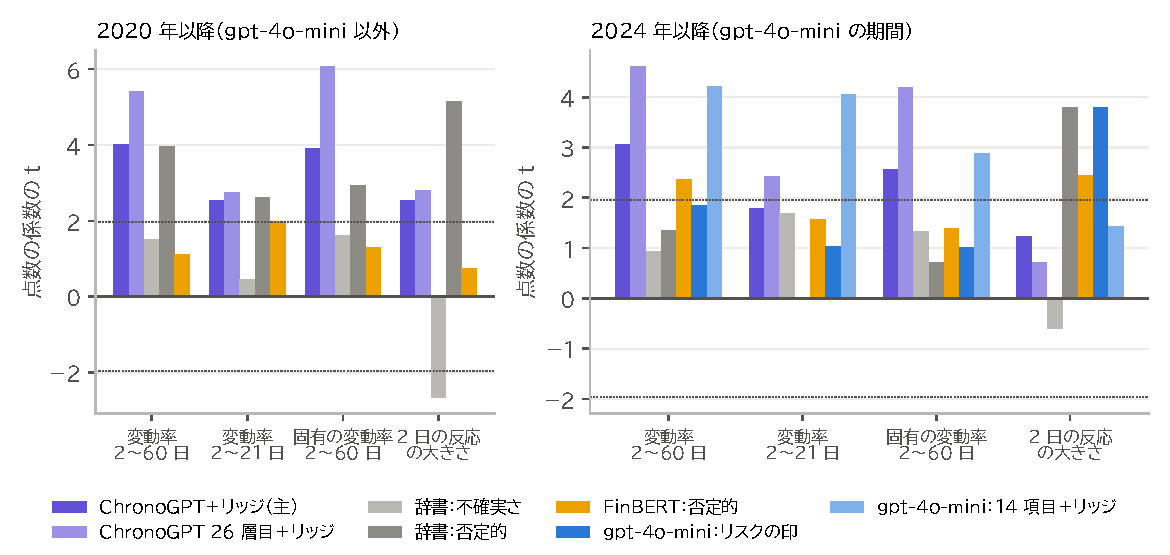
\includegraphics[width=\linewidth]{compare.pdf}
\caption{点数の係数の $t$。点線は $\pm 1.96$。}
\label{fig:compare}
\end{figure}

\begin{itemize}
\item 学習ありの点数（ChronoGPT の 2 つ、gpt-4o-mini の 14 項目）は、2〜60 日・2〜21 日・固有の変動率のどれでも正だった。
\item \textbf{2 日の反応の大きさ}は、学習なしの点数のほうがよく説明した。辞書の否定的な語、gpt-4o-mini のリスクの印の数、FinBERT の否定的な文（2024 年以降）は、反応が大きくなることを予測した。一方、辞書の不確実さの語は、2020 年以降では反応が\textbf{小さい}ことと関係した。悪い知らせを多く含む発表ほど、株価が大きく動く。
\end{itemize}

% ============================================================
\chapter{標本外の予測}\label{ch:forecast}

事前登録の副次の 4：2020 年以降の各四半期について、その四半期の前に 60 日の窓が閉じた発表だけで最小二乗を学習し、2〜60 日の変動率（対数）を予測した。基準のモデル（発表の前の変動率、規模、2 日の反応の大きさ、驚きの大きさ）と、それに ChronoGPT＋リッジの点数を足したモデルを比べた。

\begin{table}[H]
\centering\small
\caption{標本外の予測の比較（発表 \V{Fn} 件）}
\label{tab:forecast}
\begin{tabular}{@{}lr@{}}
\toprule
標本外の決定係数（基準のモデル） & \V{Fbase}\% \\
標本外の決定係数（基準＋点数） & \V{Fwith}\% \\
差 & \V{Fgain} ポイント \\
二乗誤差の比（＋点数 ÷ 基準） & \V{Fratio} \\
損失の差（基準 − ＋点数）の平均の $t$ & \V{Ft} \\
\bottomrule
\end{tabular}
\end{table}

\begin{figure}[H]
\centering
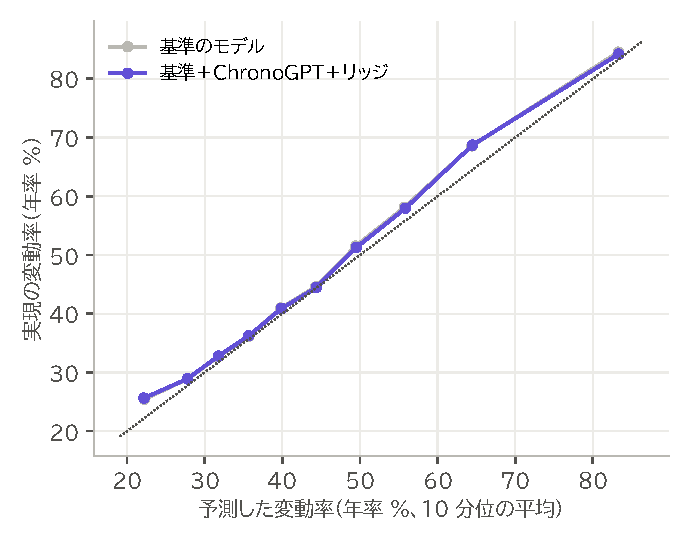
\includegraphics[width=0.6\linewidth]{forecast.pdf}
\caption{予測した変動率と実現の変動率（予測の 10 分位ごとの平均）。2 本の線はほぼ重なる。点線は予測＝実現。}
\label{fig:forecast}
\end{figure}

\begin{keybox}[結果]
発表の前の変動率などの基準のモデルだけで、標本外の決定係数は \V{Fbase}\% あった。そこに点数を足すと、予測は\textbf{わずかに悪くなった}（二乗誤差の比 \V{Fratio}、$t$ = \V{Ft}）。回帰の検定（\chapref{ch:primary}）で見えた情報は、この単純な水準の予測では役に立たなかった。
\end{keybox}

\subsection*{年ごとの内訳（実行の後に加えた記述）}

\begin{table}[H]
\centering\small
\caption{標本外の予測の二乗誤差の年ごとの平均（事前登録にない記述）}
\label{tab:forecastyear}
\tabin{forecast_year}
\end{table}

悪化は主に 2021 年に生じ、ほかの年はほぼ同じだった。2020 年は、新型コロナの急落で市場全体の変動率が予想より大きく、どちらのモデルも大きく外した（平均の誤差が大きい）。この予測のモデルは、時期の固定効果を持たないので、市場全体の変動率の水準の変化をそのまま誤差として受ける。

% ============================================================
\chapter{解釈}\label{ch:interpret}

\section{何が分かったか}

\begin{enumerate}
\item \textbf{決算発表文の読み取りは、その後の変動率を予測した}。過去の変動率と 2 日の反応の大きさを統制しても残り、置換の検定でも偶然では説明できない。2021 年以降ではより強い。
\item \textbf{ただし大きさは小さい}。1 標準偏差で変動率が約 1.5\% 高くなる程度で、変動率のばらつきの大部分は、発表の前の変動率で説明される（ヘッジファンドの報告書の第 8 章：変動率は持続性が強い）。
\item \textbf{学習ありの読み取りが効いた}。ChronoGPT のベクトルや gpt-4o-mini の 14 の項目に、変動率の驚きを正解にして重みを学習したものが強く、学習なしの点数では、辞書の否定的な語だけが効いた。
\item \textbf{水準の予測には役立たなかった}。四半期ごとに学習した単純な予測のモデルでは、点数を足すと予測がわずかに悪くなった。回帰の検定は同じ時期の銘柄どうしを比べる（時期の固定効果）のに対し、予測のモデルは水準を当てる必要があり、市場全体の変動率の変化に誤差の大部分が支配される。また、点数は四半期ごとに学習し直すリッジの出力なので、その尺度が時期によって変わる可能性がある。
\end{enumerate}

\section{BLM への使い道}

点数の情報は「同じ時期の銘柄どうしの相対的なリスク」についてのものである。BLM に使うなら、変動率の水準を置き換えるのではなく、次のような相対的な使い方が筋がよい（次の事前登録の追記の候補）。

\begin{itemize}
\item 見通しの不確かさ $\Omega$ を、リスクの点数の順位に応じて銘柄ごとに大きく・小さくする。
\item 共分散の対角（固有の分散）を、点数の順位で少しだけ補正する。
\item 発表の後、リスクの点数の高い銘柄の量を抑える。
\end{itemize}

\section{注意すべき点}

\begin{itemize}
\item 標本は今も上場している会社だけで、変動率の高い時期に消えた会社が抜けている可能性がある。
\item 変動率は日次の終値で測った。日中のデータがあれば、より正確に測れる。
\item gpt-4o-mini の期間は短い。
\item 1 回の実行の結果である。
\end{itemize}
